\chapter{Neural Network Foundations with TF}
\section{Perceptron}
The “perceptron” is a simple algorithm that, given an input vector $x$ of $m$ values $(x_1, x_2,\dots, x_m)$, often called input features or simply features, outputs either a 1 (“yes”) or a 0 (“no”). Mathematically, we define a function:
\begin{equation}
    f(x)=\begin{cases}
        1, & wx+b>0    \\
        0, & otherwise \\
    \end{cases}
\end{equation}
Where $w$ is a vector of weights, $w\cdot x$ is the dot product $\sum_{j=1}^{m}w_jx_j$ , and $b$ is the bias.
\begin{figure}
    \centering
    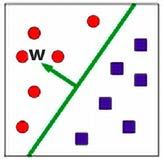
\includegraphics[width=.2\textwidth]{../img/fig1-2.png}
    \caption{An example of a hyperplane}
\end{figure}

\section{Multi-layer perceptron: our first example of a network}
\subsection{Two additional activation functions: ELU and Leaky ReLU}
Exponential Linear Unit (ELU) is defined as
$
    f(a, x)=\begin{cases}
        \alpha(e^x-1), & \text{if} \quad x \leq 0 \\
        x,             & \text{if} \quad x > 0    \\
    \end{cases}
$
for $\alpha > 0$.

LeakyReLU is defined as
$
    f(a, x)=\begin{cases}
        ax, & \text{if} \quad x \leq 0 \\
        x,  & \text{if} \quad x > 0    \\
    \end{cases}
$
for $\alpha > 0$.

\section{Multi-layer perceptron: our first example of a network}
\subsection{Further improving the simple net in TensorFlow with dropout}
这种改进背后的想法是,随机丢失迫使网络学习有助于更好泛化的冗余模式。

\subsection{Testing different optimizers in TensorFlow}
ReLU 在 0 处不可微。然而,我们可以通过将 0 处的一阶导数定义为 0 或 1,将其扩展到整个域上的函数。

ReLU 的分段导数
$\frac{\partial y}{\partial x}=
    \begin{cases}
        0, x\leq 0 \\
        1, x> 0    \\
    \end{cases}
$
\section{Regularization}
\subsection{Adopting regularization to avoid overfitting}
\figures{fig1-22}{Loss function and overfitting}
In order to solve the overfitting problem, we need a way to capture the complexity of a model, i.e. how complex a model can be. What could the solution be? \textbf{Well, a model is nothing more than a vector of weights. Each weight affects the output, except for those which are zero, or very close to it. Therefore, the complexity of a model can be conveniently represented as the number of non-zero weights.} In other words, if we have two models M1 and M2 achieving pretty much the same performance in terms of a loss function, then we should choose the simplest model, the one which has the minimum number of non-zero weights. We can use a hyperparameter $\lambda \geq 0$ for controlling the importance of having a simple model, as in this formula:
\begin{equation}
    \min:\{loss(Training~Date|Model)\}+\lambda * complexity~(Model)
\end{equation}

There are three different types of regularization used in machine learning:
\begin{enumerate}
    \item L1 regularization (also known as LASSO). The complexity of the model is expressed as the sum
          of the absolute values of the weights.
    \item L2 regularization (also known as Ridge). The complexity of the model is expressed as the sum
          of the squares of the weights.
    \item ElasticNet regularization. The complexity of the model is captured by a combination of the
          two techniques above.
\end{enumerate}
\section{A practical overview of backpropagation}
The model is updated in such a way that the loss function is progressively minimized. In a neural network, what really matters is not the output of a single neuron but the collective weights adjusted in each layer. Therefore, the network progressively adjusts its internal weights in such a way that the prediction increases the number of correctly forecasted labels. Of course, using the right set of features and having quality labeled data is fundamental to minimizing the bias during the learning process.
\figures{fig1-29}{Forward propagation and backward propagation}